%%%%%%%%%%%%%%%%%%%%%%%%%%%%%%%%%%%%%%%%%%%%%%%%%%%%%%%
%%%  Exploring the Semantic Context of News Events  %%%
%%%%%%%%%%%%%%%%%%%%%%%%%%%%%%%%%%%%%%%%%%%%%%%%%%%%%%%

\documentclass{llncs}

\newcommand{\superscript}[1]{\ensuremath{^{\textrm{#1}}}}

\usepackage{makeidx}  % allows for indexgeneration
\usepackage[hyphens]{url}
\usepackage{textcomp}
\usepackage{color}
\usepackage{listings}
\usepackage{multirow}
\usepackage{mathtools}
\usepackage{graphicx}
\usepackage{fancyvrb}
\usepackage{amsmath}
\usepackage{graphicx}
\usepackage[font=small,labelfont=bf]{caption}
\usepackage{pbox}
\usepackage{amsfonts}
\newcommand{\hg}[1]{\colorbox{yellow}{#1}}
\newcommand{\todo}[1]{\colorbox{red}{#1}}

\setcounter{MaxMatrixCols}{20}

% listing styles
\lstset{numbers=left, numberstyle=\tiny,basicstyle=\ttfamily\scriptsize, tabsize=2, keywordstyle=\underbar, stringstyle=\small, backgroundcolor=\color[gray]{0.94}, framexleftmargin=2pt}
\lstdefinestyle{rdfa}{numberblanklines=true, morekeywords={}}

%%%%%%%%%%%%%%%%%%%%%%%%
%%%  Begin Document  %%%
%%%%%%%%%%%%%%%%%%%%%%%%

\begin{document}

\frontmatter          % for the preliminaries
\pagestyle{headings}  % switches on printing of running heads
\mainmatter              % start of the contributions

%\title{Exploring the Semantic Context of News Events}
%\title{Spotting the Hidden Semantics of Newscasts}
\title{Generating Semantic Snapshots of Newscasts using Entity Expansion}
\author{Jos\'e Luis Redondo Garc\'ia\inst{2}, Michiel Hildebrand\inst{1}, Lilia Perez Romero\inst{1}, Giuseppe Rizzo\inst{2}, Rapha\"el Troncy\inst{2}}
\institute{EURECOM, Sophia Antipolis, France, \\
\email{\{redondo, giuseppe.rizzo, raphael.troncy\}@eurecom.fr}
\and
CWI, Amsterdam, The Netherlands, \\
\email{\{M.Hildebrand, L.Perez\}@cwi.nl}
}

\maketitle              % typeset the title of the contribution

%%%%%%%%%%%%%%%%%%
%%%  Abstract  %%%
%%%%%%%%%%%%%%%%%%

\begin{abstract}

% A recent trend in the newscasts domain consists on developing second screen applications that enable the user to further dive and improve his understanding of some particular news items, specially the complex word-scale controversial ones. The making of such applications requires the semantic annotation of the original newscasts as well as semantic enrichment for including background knowledge. Relying on video subtitles for providing time-based annotations of video content is a common method. However, it is insufficient to fully grasp the context of the newscasts being reported, simply because daily news reporting emphasizes on the last facts rather than on the narrative and causes of the reported event. In this paper, we propose a method that enables to search for and analyze related documents in order to generate semantic annotations that are closer to what viewers and experts in the domain expect to find while consuming newscasts. This approach generates annotations in the form of a ranked list of entities. We evaluate this method with respect to a gold standard made by domain experts for a set of BBC newscasts. Results of the experiments show the robustness in semantically annotating newscasts holding an Average Normalized Discounted Cumulative Gain of 66.4\%.

Generally newscasts in radio and television report about the latest event-related facts occurring in the world. \textit{Per se} a newscast delivers partial information thus neglecting the whole picture of the event that is often assumed as known. To rely exclusively in the broadcasted news item is therefore insufficient to fully grasp the context of the fact being reported. In this paper we propose a method that enables to retrieve and analyze related documents in order to automatically generate semantic annotations, which provide viewers and experts in the domain with more comprehensive information to fully understand the news content. On the one hand, the approach takes as inputs the publication date and the newscast's title for gathering event-related documents on the Web, bringing more representativeness to the available knowledge. On the other hand, entities spotted in subtitles are merged with those found in related documents for further disclosing hidden relevant entities that were not explicitly mentioned in the original newscast. A ranking algorithm based on entity frequency, popularity peak analysis, and domain experts' rules sorts the annotations to generate the Semantic Snapshot of the considered Newscast (SSN). We benchmark this method against a gold standard generated by domain experts and assessed via user surveys for a set of BBC newscasts. Results of the experiments show the robustness of the approach holding an Average Normalized Discounted Cumulative Gain of 66.4\%.
%Lilia: not sure whether we can call our videos newscasts or whether they are more online news videos
\keywords{Semantic Video Annotation, Entity Expansion, Newscasts}
\end{abstract}

%%%%%%%%%%%%%%%%%%%%%%%%%
%%%  1. Introduction  %%%
%%%%%%%%%%%%%%%%%%%%%%%%%

\section{Introduction}
\label{sec:introduction}
%TODO: Raphael, Michiel, to recheck and further polish research problem + hypothesis.

With the emergence of both citizen-based and social media, traditional information television channels have to re-think their production and distribution workflow processes. We live in a globalized world, a vast playing field where events happening are the result of complex interactions between many diverse agents along time. Consumers require a huge effort to interpret those news mainly because of two issues: a) the "need of background" problem: they probably need to be aware of other facts happened in a different temporal or geographical dimension, like one week ago or in a completely different region. And b), the "need of completeness" problem: a single representation of an event is not enough to capture the whole picture, because it is normally incomplete, can be biased, or partially wrong. 

In addition, traditional text-based products are losing market share against other audiovisual solutions, in particular video. In this situation, users have access to multiple news portals, which provide online access to different sources and services for commenting and debating on the news, and use social media to instantaneously spread news information. This results in large amounts of unreliable and repeated information, leaving the user exploring on their own to try to build their version of a news event from large amounts of potentially related information and trying to find the truth in the middle of an ocean of rumors or hoaxes.

The set of entities obtained from a traditional named entity extraction operation is insufficient and incomplete for expressing the context of a news event  [REF]. Sometimes entities spotted over a particular document are not disambiguated because the textual clues surrounding the entity are not precise enough for the name entity extractor.  while in other cases, they are simply not mentioned in the transcripts while being relevant for understanding the story. [LILIA]. This is also an inherent problem in information retrieval tasks: a single description about the same resource does not necessarily summarize the whole picture.

[FIGURES: recall in every source: sub, ocr, etc]

The named entity expansion operation relies on the idea of retrieving and analyzing additional documents from the Web where the same event is also described. By increasing the size of set of documents to analyze, we increase the completeness of the context and the representativeness of the list of entities, reinforcing relevant entities and finding new ones that are potentially interesting inside the context of that news item. The final result is a ranked list of entities called NewsCast Semantic Snapshot (NSS) which expands the initial set of recognized entities with more relevant concepts that help to capture the whole context of the depicted event. The NSS can be later use to feed second screen applications assisting the viewer who watches the news, summarizing and generating quality snippets, or launch further  enrichment processes who bring related content the users could be also interested in watch. 

The paper is organized as follows: Section~\ref{sec:RelatedWork} presents related work, Section~\ref{sec:ConceptExpansion} illustrates the whole method of Entity Extraction, focusing in the Collection of related documents, annotation of documents and entity filtering. Section~\ref{sec:Ranking} describes in depth the different ranking algorithms used for ordering the list of candidates entities generated in previous steps. Section~\ref{sec:Evaluation} explains the details of the ground truth, the measures considered in the evaluation, and the performance of out approach for different collection, filtering and ranking configurations, in order to see how better we are compared to the baseline and how close to the gold standard we can get. Finally Section~\ref{sec:Evaluation} summarizes the outcomes of the paper and describes our future work.

% State of the Art on Semantic annotation
* State of the Art on Semantic annotation.
Concerning the multimedia annotation the literature covers a wide range of different analysis techniques~\cite{ballan2011event}. One of the main approaches consists on running Named Entity Recognition (NER) over the textual information attached to particular video fragment. Those techniques are an essential component within the Information Extraction field that focus on: identifying atomic information units in texts, named entities; classifying entities into predefined categories (also called context types) and linking to real world objects using web identifiers (Named Entity Disambiguation). A growing number of APIs provide such a service, like AlchemyAPI\footnote{\fontsize{8pt}{1em}\selectfont \url{http://www.alchemyapi.com/}} or DBpedia Spotlight\footnote{\fontsize{8pt}{1em}\selectfont \url{http://spotlight.dbpedia.org/}}. 

%%%%%%%%%%%%%%%%%%%%%%%%%
%%%  2. Related Work  %%%
%%%%%%%%%%%%%%%%%%%%%%%%%
\section{Related Work}
\label{sec:RelatedWork}

%Studies on second screen applications and tools for supporting journalists. (WHY)
Television content in general and newscast in particular need the assistance of innovative applications which help the viewers and experts to get the most of them. One implementation design that has been deeply studied in the last years, mainly due to the increasing availability of tablets and tactile device is the "second screen application" paradigm. This kind of experiences open new possibilities for users watching television by complementing what is being displayed on the screen and offering a more active interaction with the content. In\cite{Courtois2012} the authors tracked 260 tablet users, concluding that even there is only a modest uptake and interest in using secondary screens to digitally share opinions, (other devices such as smartphones are preferred), the use of second screen interaction with television content is something the viewer qualitatively appreciate. We have also experimented the benefits of second screen applications via some prototypes like\cite{Redondo2014} which has revealed the great potential for browsing the so called "context" of the newscasts. The same concept\footnote{\fontsize{8pt}{1em}\selectfont \url{https://vimeo.com/119107849}} has been presented to the forum Iberoamerican Biennial of Design (BID)\footnote{\fontsize{8pt}{1em}\selectfont \url{http://www.bid-dimad.org/}} with great reviews from the experts and scoring between the final 5 from a total of 200 candidates. On the other hand profesional journalists also require assistance in their daily activity. Specialized researches like\cite{gynnild2014} highlight the importance of multifaceted development of algorithms, data, and social science methods in reporting and storytelling, under the term of computational exploration in journalism (CEJ). CEJ demands tools supporting the journalistic co-creation of quantitative news projects that transcend geographical, disciplinary, and linguistic boundaries.

%Entities in making sense (Semantic snapshot)  (WHAT)
All those news applications and tools need to be fed with the appropriate data to effectively assist viewers and professionals, and this information is normally broader than the one explicitly offered by the content itself. The hypothesis presented in this research paper states that this required knowledge can be represented in the form of a list of s named entities called News Semantic Snapshot (SSN) which intends to describe the context of a newscast. This idea of using semantic annotations and named entities in particular is not new. In the context of the journalism activities, projects like NEWs have studied how to disambiguate named entity in the news domain by continuously learning while processing news streams\cite{Fern�ndez2012}. In the domain of Social Networks, entities are also used for identifying and modeling events and detecting breaking news. In \cite{Steiner2013} the authors emphasize the importance of spotting news entities in short user generated post in order to obtain a better understanding about what they are talking about. Entities have been also proven to be useful in producing good results in video classification when the textual information attached to a video contains temporal references (e.g. subtitles) Yunjia et al.~\cite{yunjia2013}. 


%How to create this semantic snapshot (Expansion idea) (HOW)
In order to build a comprehensive NSS the knowledge expressed in the newscast has to be extended with more information. Our approach performs a so called Entity Expansion process, which allows to collect on the fly additional documents in the Web describing the same event. In the literature there are already some approaches relying in similar expansion techniques, even the final objetive is not spotting other event-related entities: instead, they pursue to pass from small number of named entities with the same type or category to a more complete named entity set. One of then is Google Sets \url{http://googlesystem.blogspot.fr/2012/11/google-sets-still-available.html}, an online service which is not longer available since 2014. Set expansion using the web is also closely related to the problem of unsupervised relation learning from the web\cite{Cafarella2005}, and set-expansion-like techniques have been used to derive features for concept-learning\cite{Cohen2000}, to construct �pseudo-users� for collaborative filtering\cite{Cohen99}, and to compute similarity between attribute values in autonomous databases\cite{Wolf2007}.

In 2007, RC.Wang and W.Cohen have been proposed their Set Expander for Any Language (SEAL) approach \cite{Wang2007}. SEAL works by automatically finding semi-structured web pages that contain lists of items and the aggregating these list in a way that the most promising items are ranked higher. SEAL is a language-independent system has shown good performance against previously published results like the already mentioned Google Sets. By using particular seeds and the top one hundred documents returned by Google, SEAL achieved 93\% in average precision in dataset from various languages. The same authors published an improved version of the algorithm one year later\cite{Wang2008} which increases the performance by handling unlimited number of supervised seeds. In each iteration, it expands a couple of randomly selected seeds while accumulating statistics from one iteration to another. Our approach does not rely in such kind of iterative mechanism, and focus more in maximize the quality of the search query for obtaining the most appropriate set of related documents to be analyzed.
 
Another approach in extending set of entities is \cite{Mai-Vu2010}, which combines the power of semantic relations between language terms like synonymy and hyponymy and grammar rules in order to find additional entities in the Web sharing the same category that the ones provides as input. Relying in Google they analyze documents for parsing semistructured text elements like tables and rank the final candidates using different ranking algorithms like PageRank. Several researchers propose a set expansion method using free text rather than semi-structured Web documents; for instance authors in \cite{Talukdar2006} presented a method for automatically selecting trigger words to mark the beginning of a pattern, which is then used for bootstrapping from free text. But still this approach looks for category related entities while in our case the driving force is more the event being shown in the news item.

Finally, an first implementation of the entity expansion algorithm was presented in\cite{RedondoGarcia2014}, including much less sophisticated document collection strategy, and considering only one ranking algorithm based on pure frequency. Even there is a first attempt in using DBpedia as a way to ensure the coherence of the final list of entities, there were no further efforts in use popularity measures or more elaborated rules for improve the accuracy of the results.

%%%%%%%%%%%%%%%%%%%%%%%%%%%%%%%%%%%%%%%%%%%%
%%%  3. News Concept Expansion Approach  %%%
%%%%%%%%%%%%%%%%%%%%%%%%%%%%%%%%%%%%%%%%%%%%
\section{News Concept Expansion Approach}
\label{sec:ConceptExpansion}

In this section we present our algorithm to automatically generate News Semantic Snapshots out of a particular newscast. The approach is composed of the following stages: query formulation, document collection, entity extraction, filtering strategies, entity ranking.

\begin{figure}[h!]
\centering
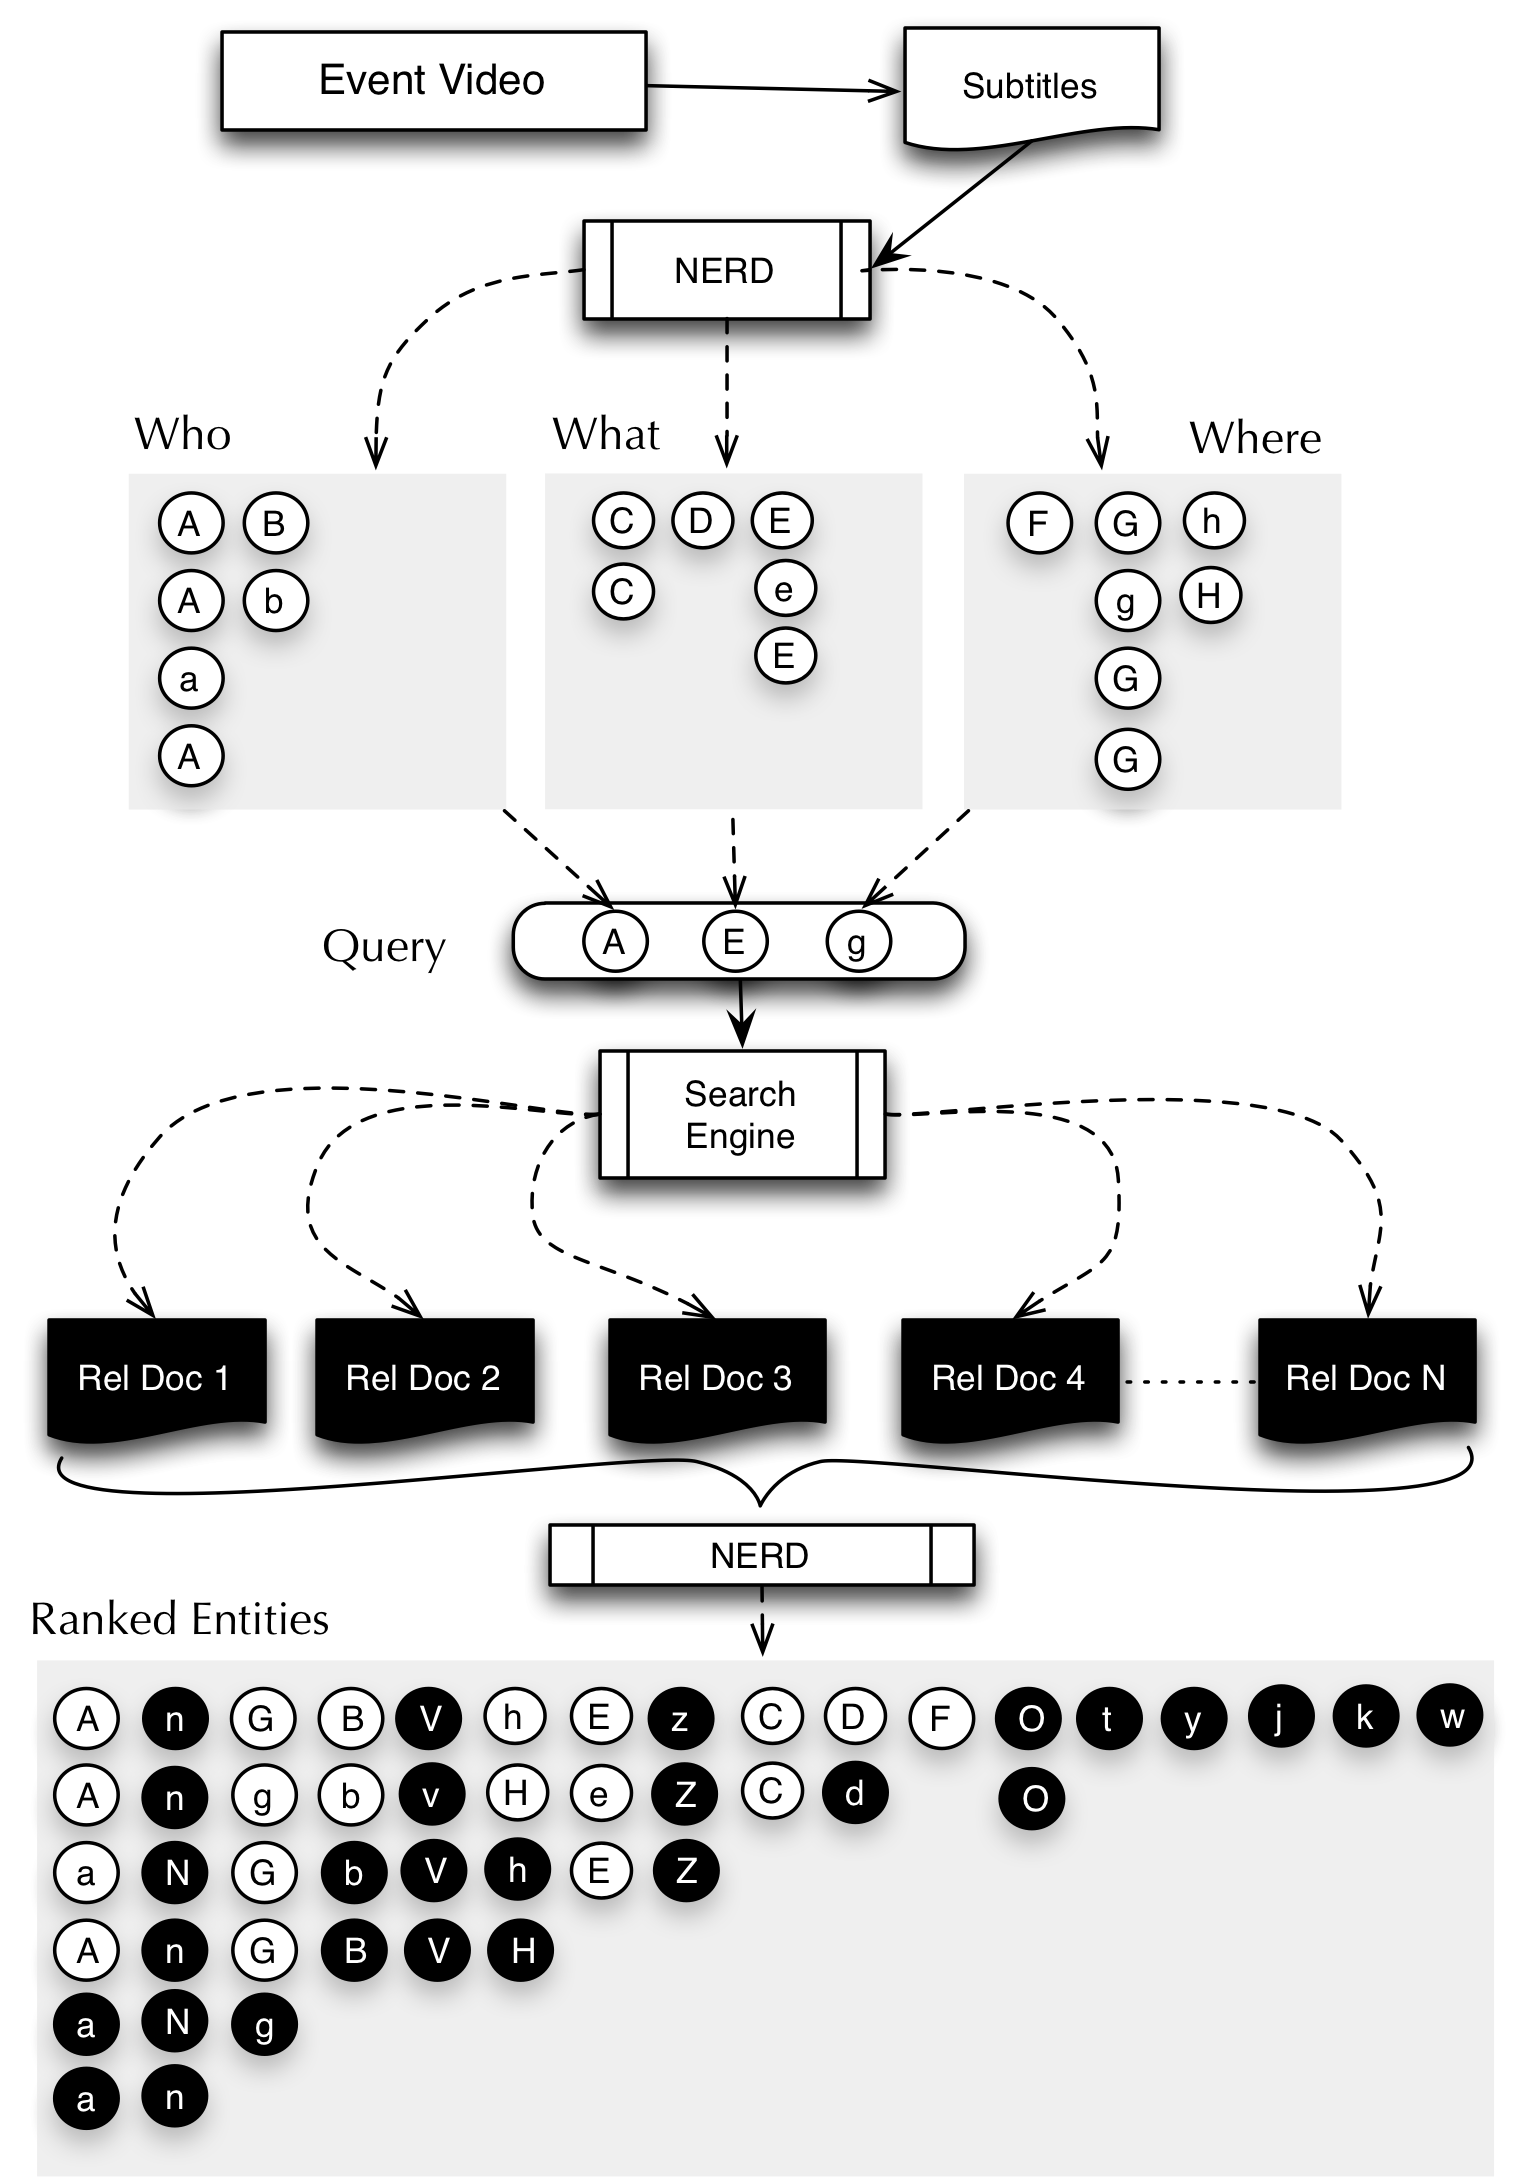
\includegraphics[width=1\textwidth]{figure/ExpansionDiagram}
\caption{Schema of Named Entity Expansion Algorithm.}
\label{fig:namedEntityExpansion}%\end{figure}
\end{figure}

\hg{GR:better to write these variables with a math formalization, i.e. lowecare, 1 letter each}

{\bf Newscast Metadata} %OLD APPROACH
%The \emph{Five W's} is a popular concept of information gathering in journalistic reporting. It captures the main aspects of a story: who, when, what, where, and why~\cite{LiJia2007}. We try to represent the news item in terms of four of those five W's (who is involved in the event, where the event is taking place, what the event is about, and when it has happened) in order to generate a query that retrieves documents associated to the same event.
%First, the original entities are mapped to the NERD Core ontology, which considers 10 main classes: Thing, Amount, Animal, Event, Function, Organization, Location, Person, Product and Time. From those ten different categories, we generalize to three classes: the Who from \url{nerd:Person} and \url{nerd:Organization}, the Where from \url{nerd:Location}, and the What from the rest of NERD types after discarding \url{nerd:Time} and \url{nerd:Amount}.
Newscast broadcasters offer a certain amount of metadata about the items they publish, which is normally available together with the audiovisual content itself. In our research, we have considered newscasts come with the following information: the title or header of the newscast, day of publication and transcript of the video (non necessary timed). In conclusion, for each newscast the following triple is needed:
\begin{equation}
\text{Event} =\left [ \text{Title}, \text{PublishingDate}, \text{Transcript} \right ]
\end{equation}

Those different fields are taken from the video publisher and directly used as input for the rest of the expansion workflow without any pre-processing.

{\bf Document Retrieval}
The first step consists of retrieving documents that report on the same event discussed in the original video. This phase in the expansion process has an key role in the upcoming filtering and ranking steps, cause it sets the basic where the rest of the algorithms will leverage on. The quality and adequacy of the collected documents sets a theoretical limit on how good the better this process is done. The more appropriate the collection of related document is, the better the final results will be.

To some extents the retrieval phase emulates what a viewer, who misses some details about the news he is watching, will do: going to the Web, make a search, and get the most of the top ranked documents. Our programmatic approach emulates this human driven task by analyzing a much bigger set of related documents in a drastically smaller amount of time. From an engineering point of view, this step consists of building a query and injecting it into a web search engine where additional descriptions about the news event can be found. This query follows the pattern:
\begin{equation}
\text{Query}_{Event} =\left [ \text{Text}, Time_{Window} \right ]
\end{equation}

Where $\text{Text}=\text{Title}$ and $Time_{Window}$ is a temporal frame containing $\text{PublishingDate}$. The middle part of Fig.~\ref{fig:namedEntityExpansion} shows this process. Those documents (colored in black in Fig.~\ref{fig:namedEntityExpansion}) will be further processed to get additional insights about the news item in the form of relevant named entities. The different behavior of search engines make some alternatives more suitable than others for certain kinds of events. The way the resulting documents change in the search engines for a particular kind of event is a research question that will not be studied in this paper. 

{\bf Semantic Annotations} Since most of the resources retrieved are Web pages, HTML tags and other annotations are removed, keeping only the main textual information. Aiming at reducing the cardinality of the textual content from the bag $D$ of retrieved documents $\{d_1, ..., d_n\}$, we perform an entity recognition analysis. The outcome of the operation is a vector of entities $E_{d_i}$ for each document $d_i$. We then consider the bag of all entities $E$ retrieved from all the analyzed documents $\{d_1, ..., d_n\}$. 

{\bf Entity Filtering} The document collection phase brings a fair number documents where relevant information about the event can be found. However this is a double-edged sword: broader number of annotations allow to build a wider view of the described event, but also bring a lot of noise. A significant part of that noise comes from certain annotations detected by the NERD-ML framework, in particular to general concepts that are not Named Entities in the strict sense of the definition. From a viewer point of view and the lesson learnt during the construction of the Ground Truth, the names of Persons, Organizations and Locations are mainly the best items to be shown. The rest of less-specific and wider enclosed concepts are more vague to be displayed on a television user interface and potentially less relevant for complementing the seed content. In order to get rid of those non relevant annotations, we have created some filters $f\left (  E_{d_i}\right )\rightarrow  E'_{d_i}$ where $\left |E'_{d_i}  \right | < \left |E_{d_i}  \right |$ by relying in different strategies which are further described in section 

{\bf Ranking Concepts from Expansion}
The different related documents collected and annotated in previous steps of the expansion algorithm contain the pieces of the puzzle that will allow to re-construct the big picture of the event. Unfortunately, those pieces come wrapped together with other less important parts which are not closely related with the event in particular and need to be put aside. By ranking the concepts, we make easier to (1) identify important entities from those which are, (2) group them in the top positions in order, (3) easy get rid of those which are not relevant to the considered event.
The output is that one.

\section{Entity Ranking}
\label{sec:Ranking}

The Entity ranking is the most crucial step in the entity expansion algorithm. The unordered but filtered set of entities has to be ranked for propose prominent concepts to the viewer get rid of the long queue of entities and noise produced by during the expansion process. the selection is much more complicated. 
prioritize entities which bring something interesting from the consumer point of view. 

\todo{GR:introduce the entity ranking and explain why doing it so}

\subsection{Clustering Entities}
In order to calculate the frequency of a particular resource within the entire corpora, we group the different appearances of the same instance and check their cardinality. This is not a trivial task since the same entity can appear under different text labels, contain typos or have different disambiguation URL's pointing to the same resource. We performed a centroid-based clustering operation over the instances of the entities. We considered the centroid of a cluster as the entity with the most frequent disambiguation URL's that also have the most repeated labels. As distance metric for comparing pairs of entities, we applied strict string similarity over the URL's, and in case of mismatch, the Jaro-Winkler string distance~\cite{winkler2006overview} over the labels. The output of this phase is a list of clusters containing different instances of the same entity.

\subsection{Frequency-based Ranking}

Counting entities.


\subsection{Pure TF-IDF Ranking}

the TF-IDF
We have considered two ways of aggregating

\begin{figure}[h!]
\centering
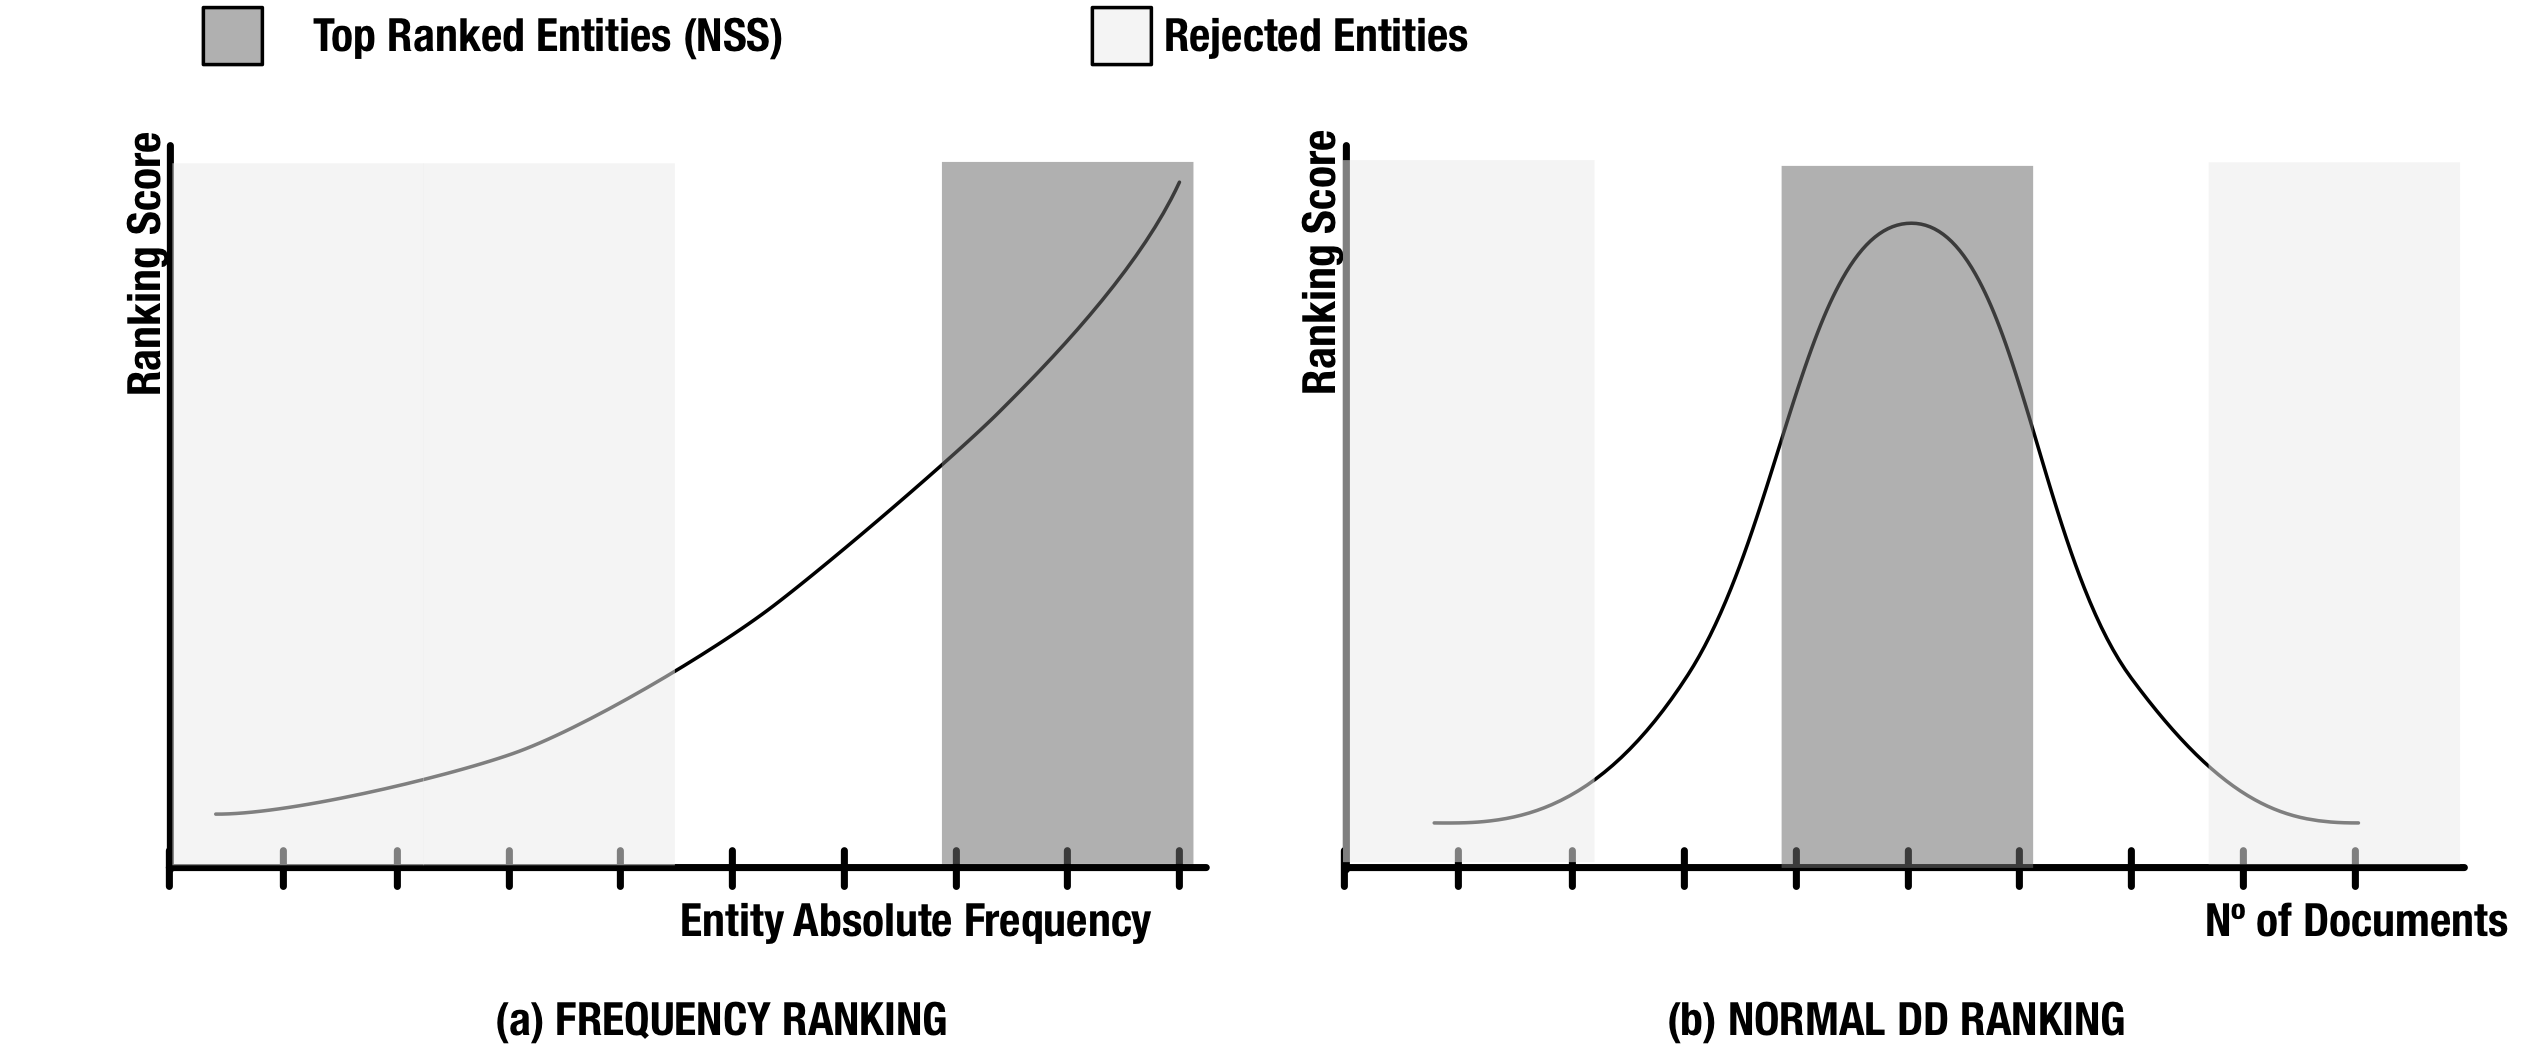
\includegraphics[width=0.9\textwidth]{figure/RankingStrategies}
\caption{Schema of Named Entity Expansion Algorithm.}
\label{fig:namedEntityExpansion}%\end{figure}
\end{figure}

\subsection{Normal distribution}

Why a normal distribution
The behavior of the users:

\subsection{Ortogonal Dimensions}

Introduction

\subsubsection{Ranking based on Popularity}

Google Trends mechanism

\begin{figure}[h!]
\centering
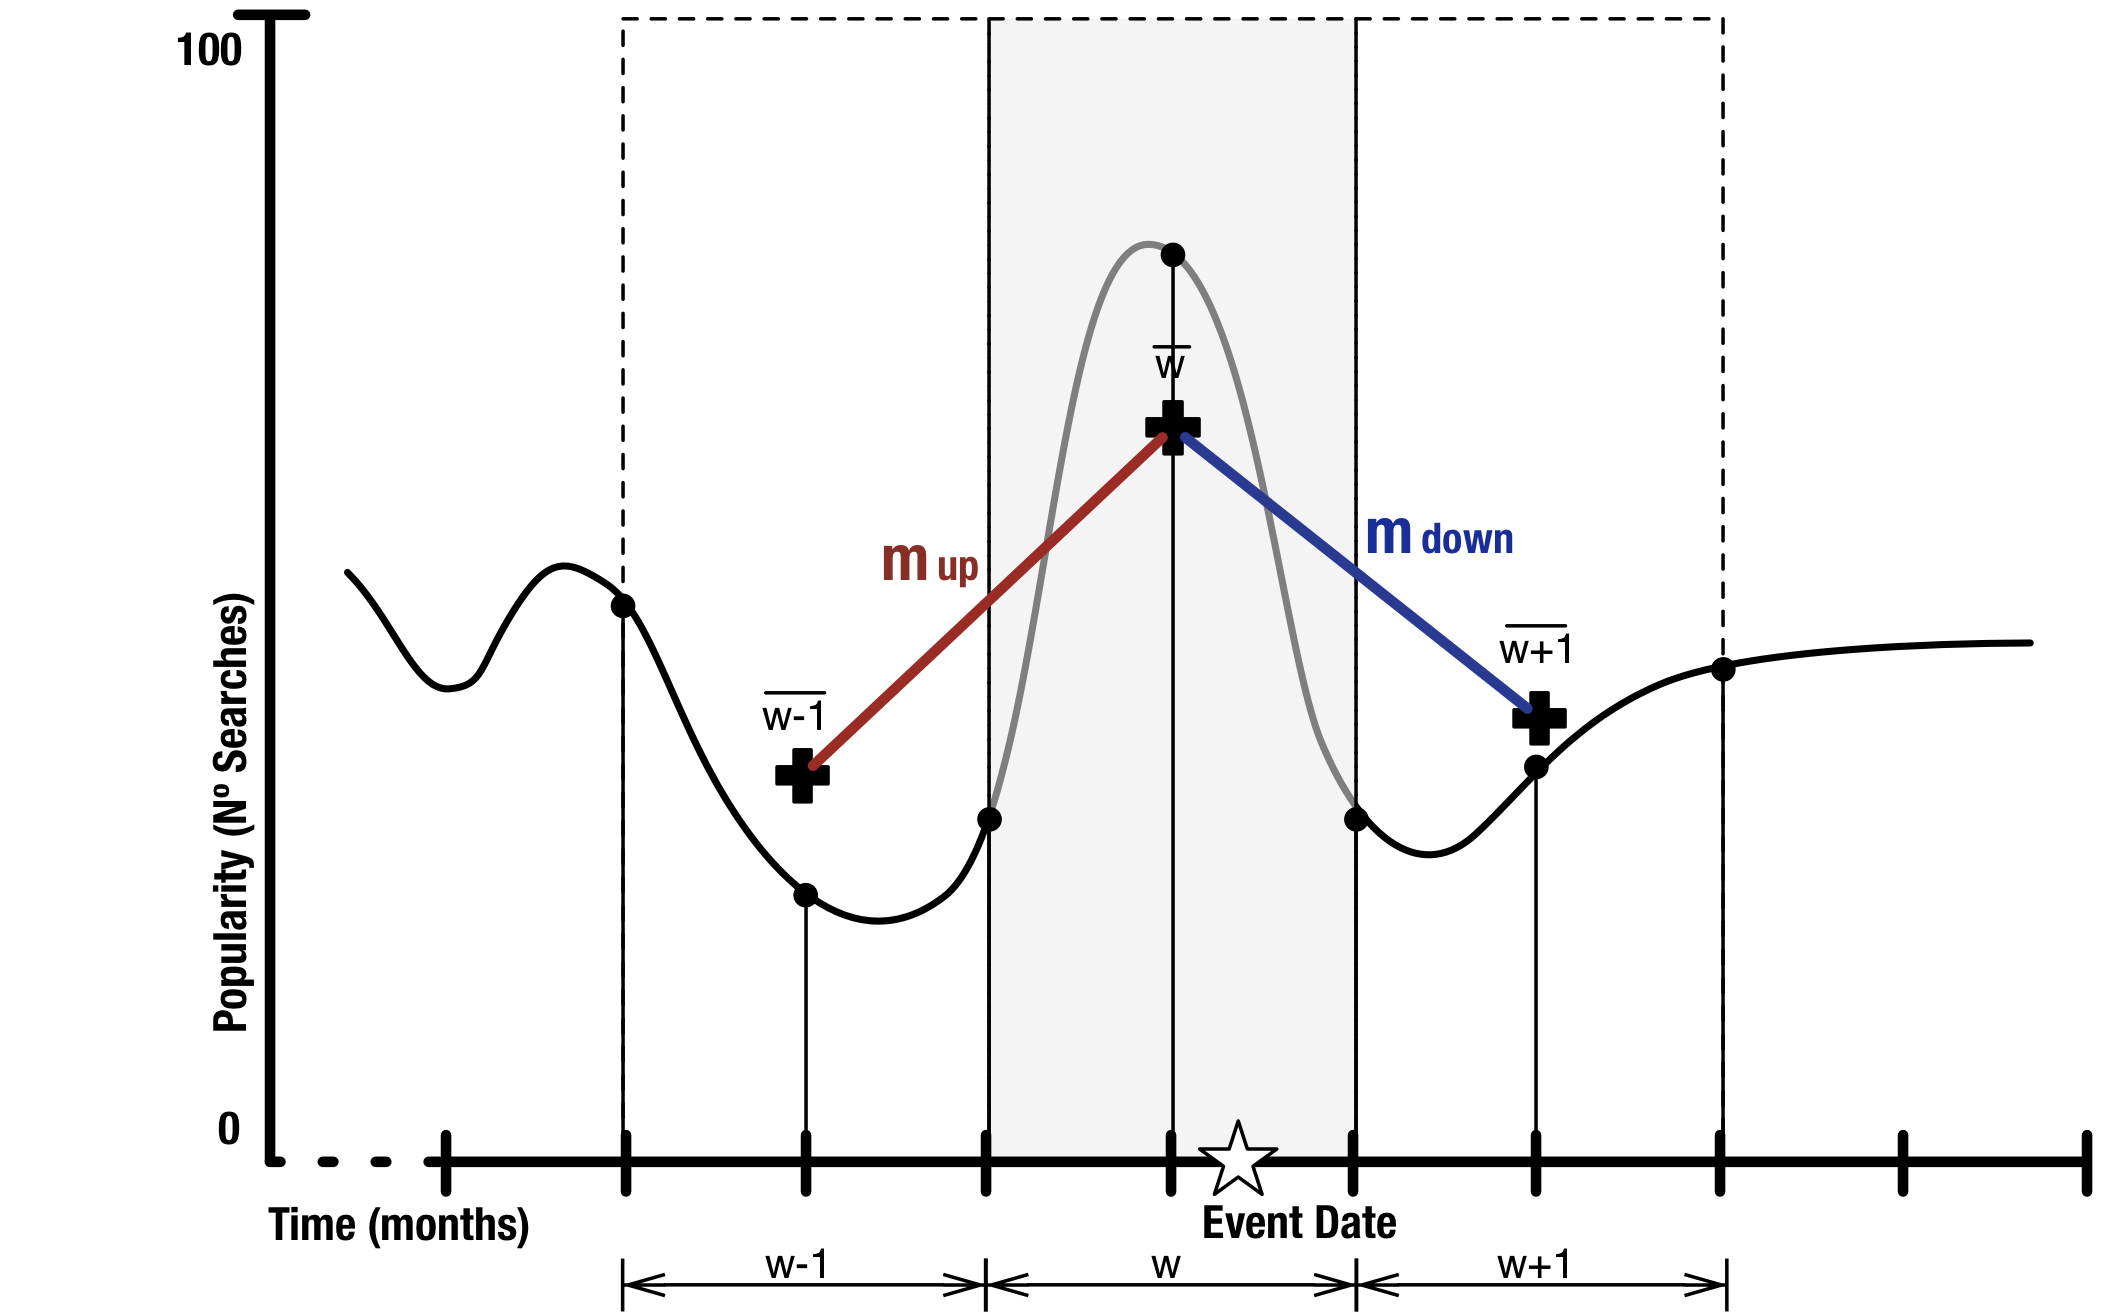
\includegraphics[width=0.7\textwidth]{figure/PopularityMeasure}
\caption{Schema of Named Entity Expansion Algorithm.}
\label{fig:namedEntityExpansion}%\end{figure}
\end{figure}

Follows a Normal distribution.

Filtering according 2sigma.

Mixing with  previous popularity

Examples
Laura Poitras
Booz Allen


% Random Walks
% PageRank
% Use prior knowledge graph

\subsubsection{Expert Rules}
Based in the conclusions from Lilia's report. 

In her study, Lilia has indicated how certain NERD types are preferred by users:
- Most of the Organizations were interesting (figures in Excel file)
- Persons
- Normally less interested in Places and other NERD categories.
- Selected by at least 2 sources.


Coeficient.

%\subsection{Pareto}

%%%%%%%%%%%%%%%%%%%%%%%%%%%%%%%%%%%%%%%%%%%%%%%%
%%%  5. Experimental Settings and Evaluation %%%
%%%%%%%%%%%%%%%%%%%%%%%%%%%%%%%%%%%%%%%%%%%%%%%%
\section{Experimental Settings and Evaluation}
\label{sec:Evaluation}
\todo{GR:main outcome in a few words, and then list the different points}
We were able to reproduce the 0.66 of Cumulative Gain by configuring the solution. Create a ground truth. In addition, we demonstrate that we are able to go further 

\subsection{Ground Truth}
\subsection{Preprocessing of the video and preparation of the candidate set}

We selected 5 short videos from the BBC One Minute World News website\footnote{\url{http://www.bbc.com/news/video_and_audio/}}. Each video lasted from 1 to 3 minutes. The selection covered a wide range of subjects specifically: politics, armed conflicts, environmental events, legal disputes, and social news. The intention behind this topic choice was to fit international audiences, since we planned to perform a user study with international participants. 

Subtitles of the videos were not available; therefore, a member of the team manually transcribed the speech in the videos.  After obtaining the transcriptions, the following steps were performed in order to obtain a set of unbiased candidate entities. We only looked for entities of the types: person, organization and location as we estimated that these three main types are the ones that can provide the most relevant information related to the news.  

\subsubsection{Subtitles}
All entities of the type person, organisation and location were manually extracted from each one of the video subtitles and added to the unfiltered list of entities (candidate set). 

\subsubsection{Image in the video}
The video image was visually analysed by a researcher and every time a recognisable person, organisation or location was portrayed this was also added as an entity to the candidate set. 

\subsubsection{Text in the video image}
The video was analysed for text appearing in the image. Whenever text appeared in the video image, for example in the form of nametag overlays, the named entities appearing in such tags were added to the candidate set. 

\subsubsection{Text in the video image}
The video was analyzed for text appearing in the image. Whenever text appeared in the video image, for example in the form of nametag overlays, the named entities appearing in such tags were added to the candidate set. 

\subsubsection{Related entities }
In order to complement the candidate set with entities that might be interesting for the user, but are not necessarily found in the videos, we used the following two strategies:

\subsubsection{Suggestions of an expert}
We collaborated with a journalist with more than 6 years of experience as a writer/editor for important American newspapers and websites.  We configured an online survey to retrieve the expert’s feedback. In the survey we explained what named entities are and which types of named entities we needed. After this introduction we presented the videos to the expert. Following each one we asked him to list the named entities that, according to his criteria, would better serve the objective of showing interesting additional information to the users. The expert didn’t have access to the candidate set, and was completely free to suggest any named entity he wanted. 

\subsubsection{Related articles}
We used Google custom search to look for articles related to the video in three news sources: The Guardian, New York Times, and Al Jazeera online (English). We performed this search using the main terms in the videos’ title, for example, for “Fugitive Edward Snowden applies for asylum in Russia” we searched for  “Edward”+”Snowden”+”asylum”+”Russia”. We limited the results to +- 3 days from the day when the video was published. We chose one document from each source, the one closest in topic and time to the video. We then extracted all named entities of the types person, organization and location from the resulting documents. In order to keep the number of entities within a reasonable number for inclusion in a survey, we kept only the named entities that appeared in at least 2 related articles and dropped all the ones that only appeared in one.  The selected entities were added to the candidate set. 

\subsubsection{Refining the candidate set}
We refined the candidate set  comprised of all found entities by eliminating all duplicated named entities and standardizing names. For example, when we had “Barack Obama” as an entity and “Obama” as another entity we eliminated the shorter one and left the complete name. 
	
A total of 99 entities were obtained from all videos. For a distribution of entities among types and videos  see Table \ref{table:entitydistribution}.

\begin{table}[h]
\begin{tabular}{| p{6cm} | l| l| l| l|}
  \hline
  \textbf{Video} & \textbf{Person} & \textbf{Organisation} &\textbf{Location} & \textbf{Total} \\
    \hline
  Fugitive Edward Snowden applies for asylum in Russia & 11 & 7 & 10 & 28 \\
    \hline
 Egypt's Morsi Vows to Stay in Power & 4 & 5 & 4 & 17 \\
    \hline
 Fukushima leak causes Japan concern & 7 & 5 & 5 & 13\\
    \hline
 Rallies in US after Zimmerman Verdict & 9 & 2 & 8 & 19 \\
    \hline
 Royal Baby Prince Named George & 15 & 1 & 6 & 22 \\
    \hline
    \textbf{Total}  & 46 & 20 & 33 & 99\\
  \hline
\end{tabular}
\caption[Table caption text]{Entity distribution in candidate set}
\label{table:entitydistribution}
\end{table}

\subsection{Online Survey}
We created an online survey with the aim of gathering information about the degree of interestingness of the entities in the candidate set. Based in [REF] we define interestingness as to whether an entity is interesting, useful or compelling enough to tear the user away from the main thread of the document. 

Fifty international subjects participated in this online study. They responded an online call distributed via email and social networks. Their age range was between 25 and 54 years with an average age of 30.3 (standard deviation 7.3 years). 18 participants were female and 32 were male. Most of the participants were highly educated and 48 of them had either a university bachelor degree or a postgraduate degree. The main requisite for participation was that they were interested in the news and followed the news regularly, preferably through means that include newscasts.
During the interview participants were asked to choose at least 3 out of 5 videos according to their preferences. Then they were shown each one of the videos. After each video, they were asked to rate whether they would be interested in receiving more information about the named entities in the context of the news video and on a second screen or similar application. All the related entities from the candidate set were shown in a list with ratio buttons arranged in a similar way to a three-point Likert-scale. The possible answers were “Yes” “Maybe” and “No”. 

\subsection{Results of the online survey}
The number of respondents per video were: “Snowden” 49, “Morsi” 34, “Fukushima” 42, “Zimmerman” 27, and “Royal baby” 15.

In order to calculate the interestingness scores from the users’ responses, we gave every answer a numerical value: Yes = 1, Maybe = 0 and No = -1.  We then obtained an average score for each entity according to the number of users who answered the survey per video.  We consider that the participants responded positively, or found interesting all entities with an average score of 0 or more and discarded the rest of the entities as “not interesting”.


\subsection{Measures}
Measurements in terms of Recall and Precision, at 7 (average number of results selected as relevant by the users)
However those measures do not distinguish between differences in the rankings at positions 1 to p, which may be considered important for some tasks. For example, the two rankings in Figure 8.2 will be the same when measured using precision at 10.

This is why  the evaluation we will focus in the highly ranked relevant documents. Similar to Web search engines, we will apply an evaluation measure which will try to find as many relevant documents as possible, while still keeping the  premise that the top ranked documents are the most important. We will not perform measures in terms of efficiency. Even this kind of study is easier to quantify (most of the time it can be measured automatically with a timer instead of with costly relevance judgments) this falls outside the scope of this paper.
** How external items are measured.

Those are the key efficiency measurements we would like to perform,

** Mean average precision at 10  - single number summary, popular measure, pooled
relevance judgments.

** Average NDCG - single number summary for each rank level, emphasizes top ranked documents, relevance judgments only needed to a speciffc rank depth
(in our example 10).

** Recall-precision graph - conveys more information than a single number measure, pooled relevance judgments.

** Average precision at rank 10 - emphasizes top ranked documents, easy to understand, relevance judgments limited to top 10.

We will use the same same ranking algorithm on five different queries. We aim of an averaging technique is to summarize the effectiveness of a specific ranking algorithm across a collection of queries. Different queries will then have different numbers of relevant documents, as is the case in this example. Figure about recall-precision for the top ten rank positions.

Average between 5 queries.

SELECTING PRECISION AT N


\begin{figure}[h!]
\centering
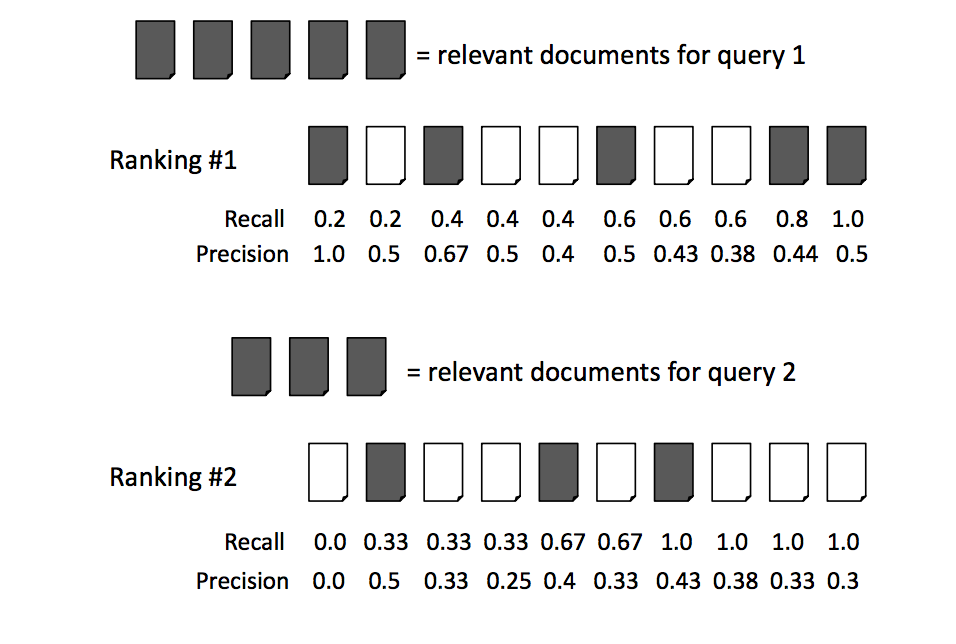
\includegraphics[width=0.9\textwidth]{figure/cumulativeGain}
\caption{Evaluation measures in document retrieval.}
\label{fig:namedCumulativeGain}%\end{figure}
\end{figure}

\subsection{Experimental Settings}
\label{sec:experimentalSettings}

\subsubsection{Document retrieval}
In this regard, we have relied on the Google Custom Search Engine API service\footnote{\fontsize{8pt}{1em}\selectfont  \url{https://www.google.com/cse/all}} by launching a query with the parameters specified in $\text{Query}_{Event}$. Apart of the query itself, the CSE engine considers other parameters that need to be tuned up. First, due to quota restrictions the maximum number of retrieved document is set to 50. As shown in the evaluation described in the Section~\ref{sec:evaluation}, this is enough for significantly extending the initial set of documents. But addition, we have also considered 3 different dimensions that could potentially influence the effectiveness in retrieving related documents:
\begin{enumerate}
 \item Web sites to be crawled. Google allows to specify a list of web domains and subdomains where documents can be retrieved from. This reduces the scope of the search task and, depending on the characteristics of the considered sources, influence the nature of the retrieved items: from big online newspapers to user generated content. At the same time, Google allows to prioritize searching over those whitelists while still considering the  whole indexed Web. Based on this, in our study we considered five possible values for this parameter:
a) AllGoogle: search over the whole set of Web pages indexed by Google.
 \begin{itemize}
  \item Newspaper whitelist. A set of 10 internationals English speaking newspapers chosen from \footnote{\fontsize{8pt}{1em}\selectfont  \url{http://en.wikipedia.org/wiki/List_of_newspapers_in_the_world_by_circulation}}
  \item Lilia's whitelist. A set of 3 international newspapers used in [Lilia] while building the ground truth used in Section~\ref{sec:evaluation}.
  \item Newspaper whiteList + Google. Prioritize content in Newspaper whitelist but still consider other sites.
  \item Lilia's whitelist + AllGoogle: Prioritize content in Lilia's whitelist but still consider other sites.
 \end{itemize}
 \item Temporal dimension. This variable allows to filter those documents which are not temporarily close from the day where the newscast was published. Assuming that the news item is fresh enough, this date of publication will also be fairly close to the day the event  took place. Taking $\text{PublishingDate}$ as a reference and increasing the window in a certain amount of days $d$,  we end up having $Time_{Window}=\left [ \text{PublishingDate}-d, \text{PublishingDate}+d \right ]$ The reason why we expand the original event period is because documents concerning a news event are not always published during the time of the action is taking place but some hours or days after or before. The final $Time_{Window}$ could vary according to many factors such as the nature of the event itself (whether it is a brief appearance in a media, or part of a longer story with more repercussion) or the kind of documents the search engine is indexing (from very deep and elaborated documents that need time to be published, to short post quickly generated by users). In this study we have considered two possible values for it: 2 weeks and one week temporal windows.
 \item In addition, Google Custom Search Engine makes possible to filter result according to the Schema.org types: 2 values:. Based on the study.
[NoFilter(Default), Person\&OrganizationFiltered]
\end{enumerate}

TABLE OF RESULTS
That makes $5 * 2 * 2 = 20$ different runs 

that we will study in the Section~\ref{sec:evaluation} in order to discover which configuration optimizes the expansion algorithm.

* Explain insights obtained from the survey. \% of entities coming from subtitles, form other sources, etc

\subsubsection{Entity Filtering}
\label{sec:settingsFiltering}

After some first trials it became evident that those many non-pure Named Entities which were not well considered by viewers and expert during the ground truth creation [Lilia] were dramatically dropping the scores for most of the considered ranking strategies. We have foreseen three different filtering approaches for getting rid of those undesired concept annotations:

\begin{enumerate}
\item Filter by type (F1). Filter annotations according to their NERD type. In our case, only \textbf{nerd:Person}, \textbf{nerd:Location}, and \textbf{nerd:Organization} entities.
\item Filter by confidence (F2). Second strategy consist on getting ride of entities with confidence score under first quarter of the distribution.
\item Filter instances (F3). Intuitively, people seems to be more attracted by proper names. Those names are normally uppercased. This filter keeps only concepts matching this rule.
\end{enumerate}

We executed different runs by applying those filters over the original annotations and their corresponding combinations, manly: (F1 - F2 - F3 - F1\_F2 - F1\_F3 - F2\_F3 - F1\_F2\_F3 ), resulting in significant improvement in the final scores as shown in Section~\ref{sec:FilteringExperiments}, in terms of different measures like Precision, recall, average precision, and NDCG.

\subsubsection{Entity Ranking}
\label{sec:settingsRanking}

All strategies considered, with and without Expert rules, with / without popularity.

\subsection{Results}


TABLE showing content. Measures

1) The problem with non strict Named Entities being promoted in TFIDF strategy is clearly alleviated for all filters and combinations. TF strategy has generally improved as well, but in a lower scale.
2) The TF strategy performs better than the current implementation of TFIDF in ALL cases.
3) Best Filter for TF strategy is F3 (0.523665971)
4) Best Filter for TFIDF strategy is the combination F1\_F3
5) I combined the results for both strategies via a) simple multiplication and b) their average value, see rows 4th and 5th. In both cases, the combination F1\_F3 seems to perform the best.


%%%%%%%%%%%%%%%%%%%%%%%
%%%  5. Conclusion  %%%
%%%%%%%%%%%%%%%%%%%%%%%

\section{Conclusion}
\label{sec:conclusion}
We presented an approach for context-aware annotating news events, designed to precisely harvest program descriptions starting from named entities recognized in TV video transcripts. Because the entities initially spotted are typically insufficient for covering the broader range of concepts that best describe a particular news clip, we expanded this set by analyzing additional textual documents about the same event.

The evaluation indicates that we can successfully expand the initial set of recognized entities with more relevant concepts not detected by pure named entity recognition approaches and produce a more accurate ranking of important concepts that brings forward entities which user are more interested about.

Future: tailor ranking to particular types of news: sport, politics, regional, international, opinion, etc. Survey on 15 videos from the BBC about international facts. Evaluated over people in different countries.
semantic annotation for doing: summarizing topics/entities


%%%%%%%%%%%%%%%%%%%%%%%%%
%%%  Acknowledgments  %%%
%%%%%%%%%%%%%%%%%%%%%%%%%

\section*{Acknowledgments}
This work was partially supported by the European Union's 7th Framework Programme via the project LinkedTV (GA 287911).

%%%%%%%%%%%%%%%%%%%%%%
%%%  Bibliography  %%%
%%%%%%%%%%%%%%%%%%%%%%
\bibliographystyle{abbrv}
\bibliography{NewsConceptExpansion}

\end{document}
